% ---------------------------------------------------------------------------- %
\chapter{Experimental Setup}
\label{chap:experimentalSetup}
% ---------------------------------------------------------------------------- %

This  chapter will  present a  brief overview  of the  hardware and  provide a
step-by-step guide to put it into operation.

% ---------------------------------------------------------------------------- %
\section{Hardware Overview}
\label{sec:hwOverview}
% ---------------------------------------------------------------------------- %

The   hardware   consists   of   two  primary   components: The   test   board
(\fref{fig:pcbOverview})and a \raspi~ (\fref{fig:raspi}).

The test board's purpose is to provide all the necessary circuitry for driving
the sensor  IC in a  convenient package. On its  left-hand side, it  has seven
industrial plugs  for connecting to  power supplies,  an input signal,  a test
output for the preamp as well as ground.

At the board's top edge, connections for the externally provided clock and the
output signal line can be found.

\begin{figure}
    \centering
    %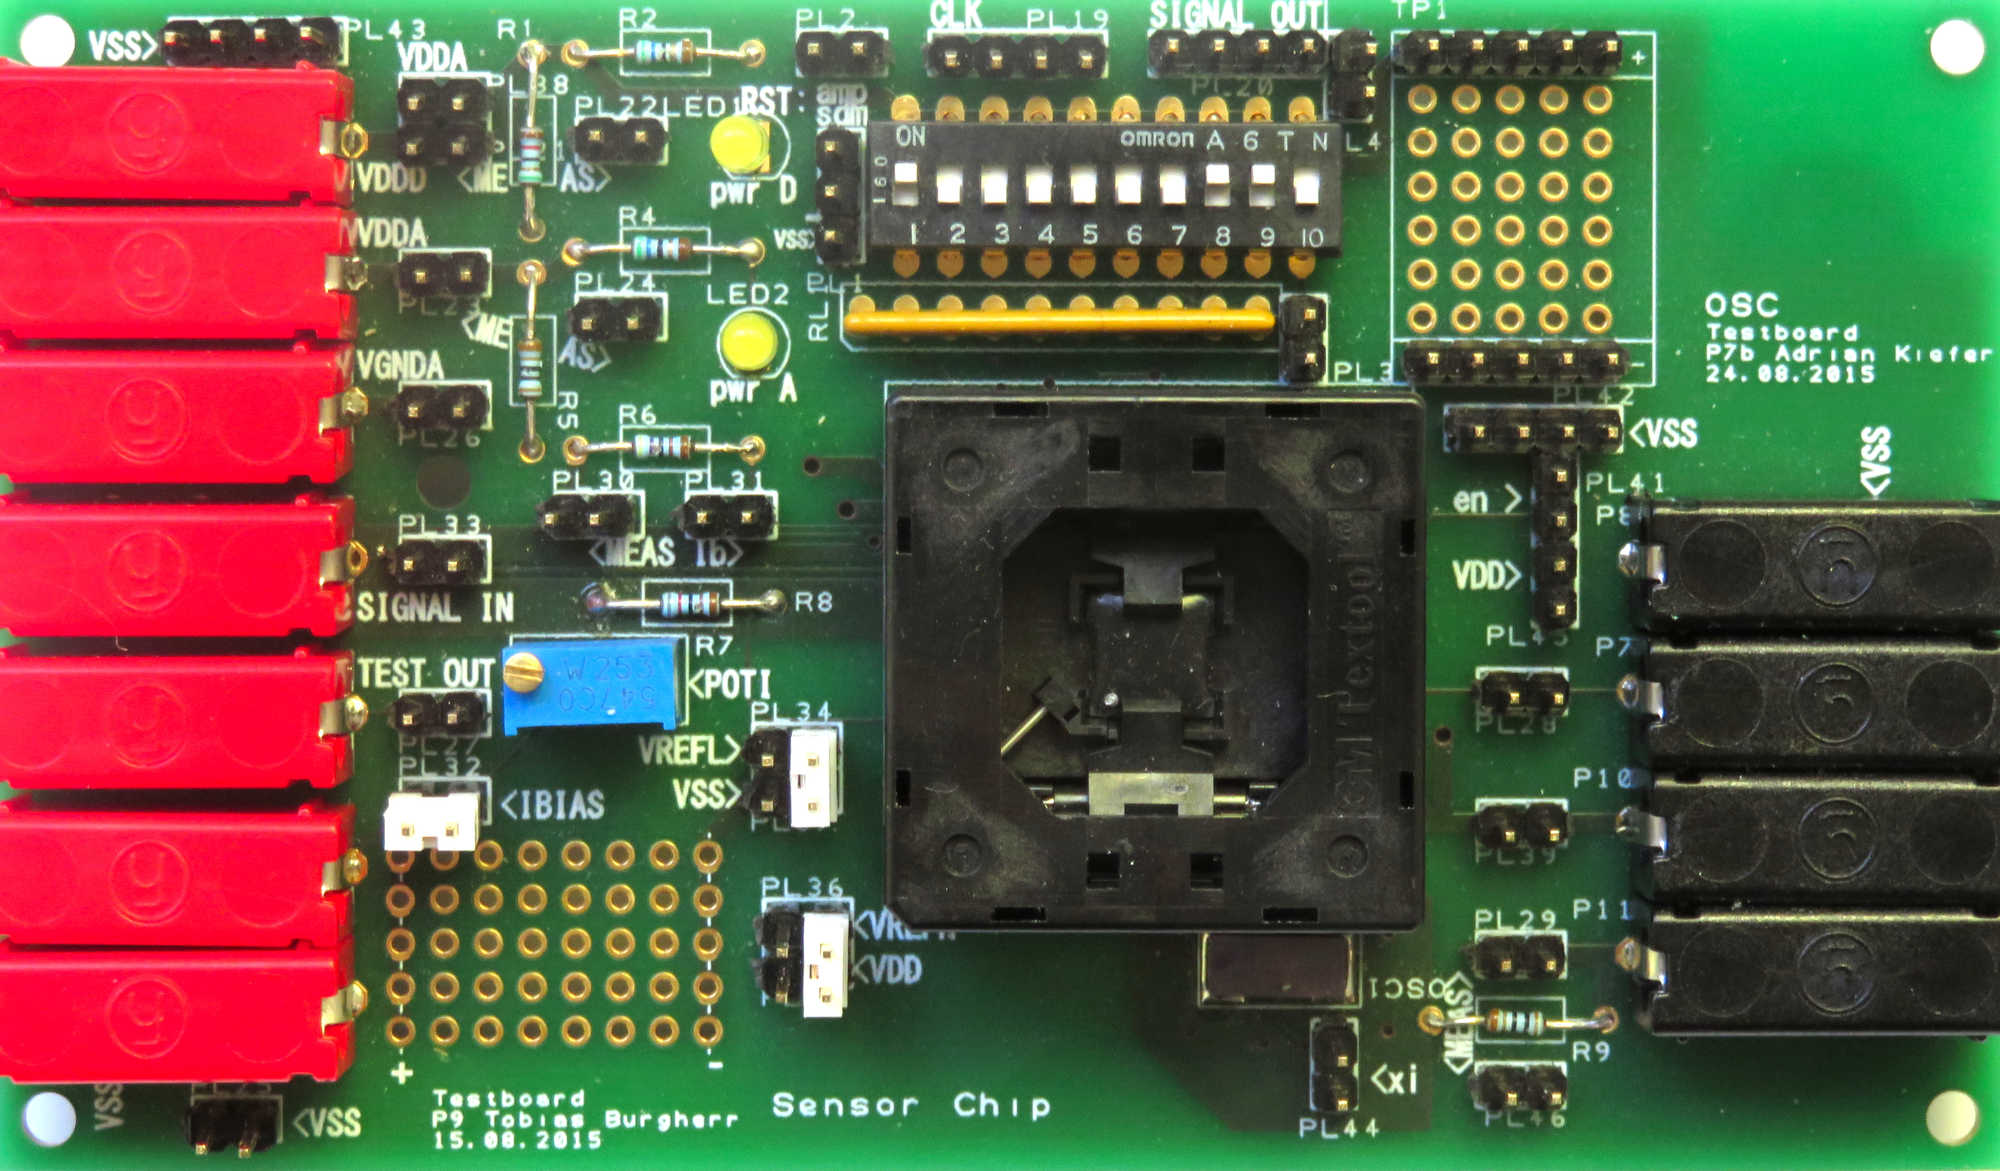
\includegraphics[width=\textwidth]{images/pcb/pcbOverview.jpeg}
    \newcommand{\plugtext}[1]{\textbf{\texttt{\Large{#1}}}}

\begin{tikzpicture}
    \begin{scope}[x={(0mm,135mm)},y={(0mm,79mm)},line width=1pt,cap=round]
        \node[anchor=south west,inner sep=0mm] at (0mm,0mm) {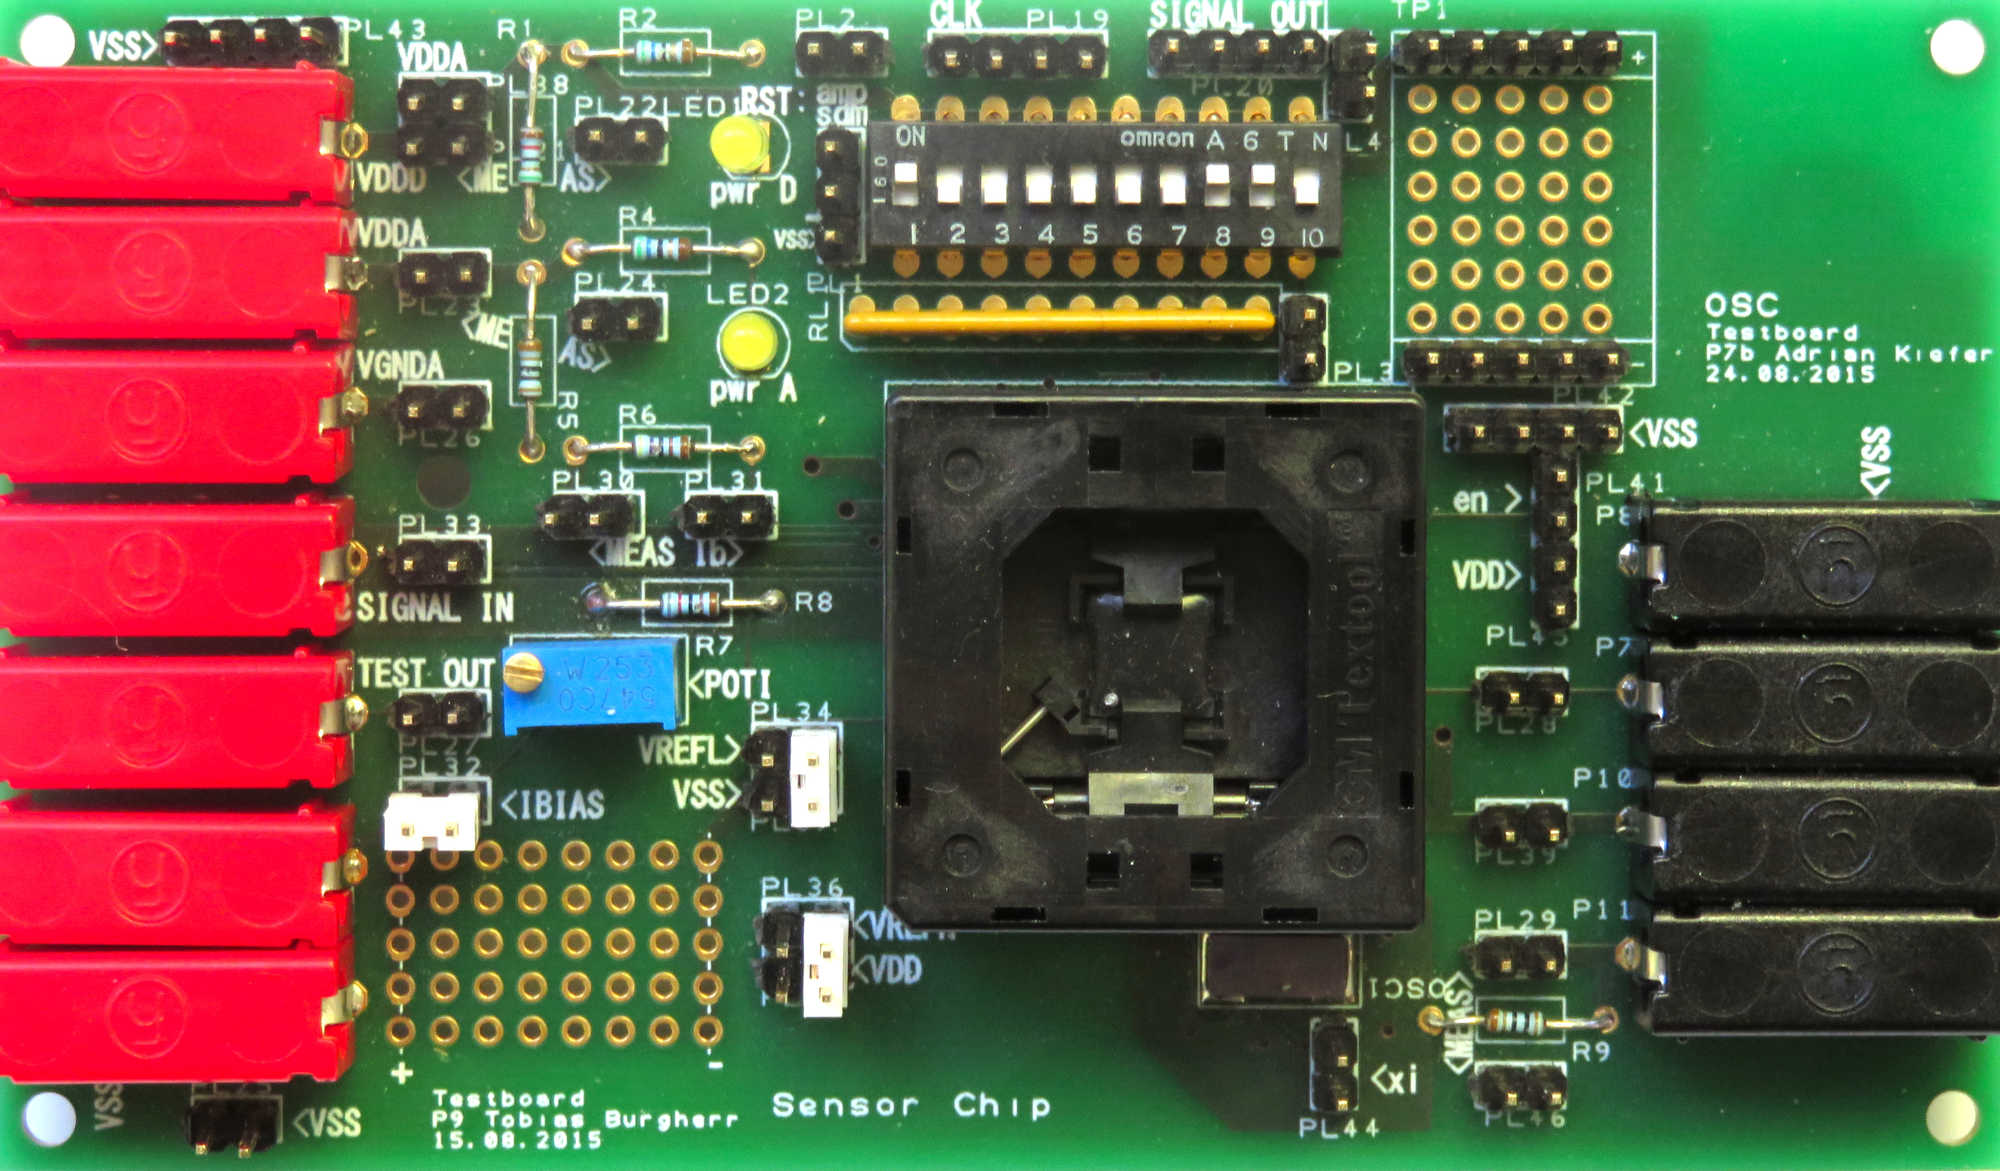
\includegraphics[width=135mm]{images/pcb/pcbOverview.jpeg}};
    \end{scope}
    %\node[fill=black,text=white,anchor=south west] at (0mm,0mm) {\textsf{\Large{VDDD}}};

    \node[%
        %fill=black,
        %fill opacity=0.5,
        text=white,
        text opacity=1,
        rounded corners=1mm,
        anchor=south west] at (4mm,66mm) {\plugtext{VDDD}};

    \node[%
        %fill=black,
        %fill opacity=0.5,
        text=white,
        text opacity=1,
        rounded corners=1mm,
        anchor=south west] at (4mm,56.5mm) {\plugtext{VDDA}};

    \node[%
        %fill=black,
        %fill opacity=0.5,
        text=white,
        text opacity=1,
        rounded corners=1mm,
        anchor=south west] at (4mm,47.5mm) {\plugtext{VGNDA}};

    \node[%
        %fill=black,
        %fill opacity=0.5,
        text=white,
        text opacity=1,
        rounded corners=1mm,
        anchor=south west] at (1mm,37.5mm) {\textbf{\textsf{\large{SIGNAL IN}}}};

    \node[%
        %fill=black,
        %fill opacity=0.5,
        text=white,
        text opacity=1,
        rounded corners=1mm,
        anchor=south west] at (1mm,27.5mm) {\textbf{\textsf{\large{TEST OUT}}}};

    \node[%
        %fill=black,
        %fill opacity=0.5,
        text=white,
        text opacity=1,
        rounded corners=1mm,
        anchor=south west] at (4mm,17mm) {\plugtext{IBIAS}};

    \node[%
        %fill=black,
        %fill opacity=0.5,
        text=white,
        text opacity=1,
        rounded corners=1mm,
        anchor=south west] at (4mm,8mm) {\plugtext{VSS}};
\end{tikzpicture}

    \caption{Test board overview with its most commonly used connections labeled}
    \label{fig:pcbOverview}
\end{figure}

\begin{figure}
    \centering
    \missingfigure{Raspberry Pi}
    \caption{The Raspberry Pi used in this setup}
    \label{fig:raspi}
\end{figure}

The chip's top  level pins are listed in  \tref{tab:inputPlugs}. Some of these
can  be configured  via an  array of  DIP switches,  located between  the chip
socket  and  the  \signal{CLK}  and  \signal{SIGNAL OUT}  plugs  on  the  test
board. The most commonly  used among these is the preamp's  gain, which can be
set to values between \num{-16}  and \num{+16}. The preamp's sign (positive or
negative) is  a dedicated  switch; its  gain's absolute  values are  listed in
\tref{tab:dipGain}.

\begin{table}
    \centering
    \caption{Sensor chip toplevel pins}
    \label{tab:inputPlugs}
    \scriptsize
    \sisetup{list-pair-separator = { or }}
    \rowcolors{2}{solarized-base3}{white}
    \begin{tabular}{>{\fontfamily{jkptt}\selectfont}l>{\fontfamily{jkptt}\selectfont}lp{30mm}lp{30mm}} \\
    %\begin{tabular}{>{\fontfamily{lmtt}\selectfont}l>{\fontfamily{lmtt}\selectfont}lp{30mm}lp{30mm}} \\
        \toprule
        \textnormal{\textsc{Pin \#}} & \textnormal{\textsc{Name}}                  & \textsc{Description} & \textsc{Value} & \textsc{Note} \\
        \midrule
        39 & vin                     & analog input signal                         & \SIrange{0.5}{2.5}{\volt} & \\
        25 & bit\_stream             & digital output signal                       & \SIlist{0;3}{\volt}       & \\
        34 & clk                     & clock                                       & \SIlist{0;3}{\volt}       & \\
        36 & sdm\_rst                & pulse to reset the $\Sigma\Delta M$         & \SIlist{0;3}{\volt}       & short pulse is enough (min $T_C$) \\
        41 & vgnda                   & analog ground                               & \SI{1.5}{\volt}           & \\
        48 & vrefh                   & high reference voltage                      & \SI{3}{\volt}             & \\
        47 & vrefl                   & low reference voltage                       & \SI{0}{\volt}             & \\
        46 & ibias                   & bias current                                & \SI{120}{\micro\ampere}   & $24 \cdot 5 \cdot 1$, internally reduced by 120 \\
        43 & sc\_amp\_vout\_test\_en & enables test output after preamp            & \SIlist{0;3}{\volt}       & \SI{0}{\volt}: off, \SI{3}{\volt}: on\\
        44 & sc\_amp\_vout\_test     & test output after preamp                    & \SIrange{0.5}{2.5}{\volt} \\
        33 & sc\_amp\_rst\_ext\_en   & enables external reset input for the preamp & \SIlist{0;3}{\volt}       & \SI{0}{\volt}: off, \SI{3}{\volt}: on\\
        32 & sc\_amp\_rst\_ext       & external reset input for the preamp         & \SIlist{0;3}{\volt}       & Internally synced to \signal{clk}. Needs \signal{en} signal. \\
        35 & sc\_amp\_pos\_neg\_amp  & positive or negative gain                   & \SIlist{0;3}{\volt}       & \SI{0}{\volt}: positive, \SI{3}{\volt}: negative \\
        28 - 31 & sc\_amp\_csel<3:0> & set gain                                    & \SIlist{0;3}{\volt}       & See table TODO \\
        27 & sc\_amp\_en             & enable preamp                               & \SIlist{0;3}{\volt}       & \SI{0}{\volt}: off, \SI{3}{\volt}: on\\
        26 & sah\_sdm\_en            & enable $\Sigma\Delta M$ S/H bock            & \SIlist{0;3}{\volt}       & \SI{0}{\volt}: off, \SI{3}{\volt}: on\\
        42 & vdda                    & analog positive power supply                & \SI{3}{\volt}             & \\
        37 & vddd                    & digital positive power supply               & \SI{3}{\volt}             & \\
        40 & vss                     & analog and digital negative power supply    & \SI{0}{\volt}             & \\
        \bottomrule
    \end{tabular}
    \sisetup{list-pair-separator = { and }}
\end{table}

\begin{table}
    \centering
    \caption{DIP switch settings for amplifier gain}
    \label{tab:dipGain}
    \scriptsize
    \begin{tabular}{%
            >{\fontfamily{jkptt}\selectfont}r
            >{\fontfamily{jkptt}\selectfont}r
            >{\fontfamily{jkptt}\selectfont}r
            >{\fontfamily{jkptt}\selectfont}r|
            >{\fontfamily{jkptt}\selectfont}r}
        \toprule
        \signal{sc\_amp\_en(3)} &
        \signal{sc\_amp\_en(2)} &
        \signal{sc\_amp\_en(1)} &
        \signal{sc\_amp\_en(0)} &
        Gain \\
        \midrule
        1 & 1 & 1 & 1 &  1 \\
        0 & 1 & 1 & 1 &  2 \\
        0 & 0 & 1 & 1 &  4 \\
        0 & 0 & 1 & 1 &  8 \\
        0 & 0 & 0 & 1 & 16 \\
        \bottomrule
    \end{tabular}
\end{table}


% ---------------------------------------------------------------------------- %
\clearpage
\section{Putting the Sensor IC Into Operation}
\label{sec:ICintoOperation}
% ---------------------------------------------------------------------------- %

This  section  will  detail  the  steps  needed to  put  the  Sensor  IC  into
operation. Some  of  this  information  will be  redundant  with  the  reports
\cite{ref:burgherr},  \cite{ref:gloor} and  \cite{ref:baier},  but  we aim  to
provide a  convenient guide for this  process in a single  place, thus sparing
future teams the effort of needing  to assemble this information from multiple
sources, which is both a time-consuming and error-prone process.
\todo[noline]{Make direct references to pages/tables in other reports?}
\todo[noline]{Safety precations}

Fundamentally, putting the chip into operation consists of the following steps:
\begin{itemize}\tightlist
    \item
        Set up \raspi.
    \item
        Determine bias resistor setting.
    \item
        Set   DIP   switches   to   the  appropriate   values   according   to
        \tref{tab:dipGain}.
    \item
        Connect supply voltages and bias current supply.
    \item
        Connect \raspi~and test board.
\end{itemize}

% ---------------------------------------------------------------------------- %
\subsection{Setting up the Raspberry Pi}
\label{subsec:raspiInstall}
% ---------------------------------------------------------------------------- %

\todo[inline]{%
    Give a more detailled guide on what to install on the \raspi~ and how than
    in the previous reports
}

\todo[inline]{RaspiPower supply}
\todo[inline]{External connections for Raspi}
\todo[inline]{%
    Controlling the  function generator  for \signal{SIGNAL  IN} line  via the
    \raspi.
}

% ---------------------------------------------------------------------------- %
\subsection{Hardware Setup}
\label{subsec:hardwareSetup}
% ---------------------------------------------------------------------------- %

Operating the test board requires the following components:

\begin{itemize}\tightlist
    \item
        direct voltage source: \SI{3}{\volt}
    \item
        direct voltage source: \SI{1.5}{\volt}
    \item
        Direct  current  source: \SI{120}{\micro\ampere}.  \emph{Note:} If  no
        direct current source  is available, as in our case,  a direct voltage
        source in combination with  a multimeter for controlling/measuring the
        current can be used.
    \item
        function generator for \signal{clk}
    \item
        Direct  and  alternating  voltage  source  for  input  signal  voltage
        (between \SI{0.5}{\volt} and \SI{2.5}{\volt}).
    \item
        An oscilloscope for monitoring the preamp's output on the \signal{TEST
        OUT} pin, as well as the raw bit stream.
\end{itemize}

The complete setup is depicted in \fref{fig:experimentDiagram}.

\begin{figure}
    \sisetup{range-phrase = { \ldots }}
\sisetup{list-pair-separator = {/}}

\begin{circuitikz}[x=1mm,y=1mm]

    % ------------------------------------------------------------------------ %
    % Test Board
    % ------------------------------------------------------------------------ %
    \draw (0,0) -- (50,0) -- (50,29) -- (0,29) -- cycle;

    % Left-hand side Plugs
    \foreach \y in {0,...,6} {%
        \draw (0,\y*3.5+2.5) -- (8,\y*3.5+2.5) -- (8,\y*3.5+5.5) -- (0,\y*3.5+5.5) -- cycle;
    };

    % CLK plug
    \draw (23,27.5) -- (27,27.5) -- (27,28.5) -- (23,28.5) -- cycle;
    \foreach \x in {0,...,3} {%
        \fill (23.25+\x,27.75) -- (23.25+\x+0.5,27.75) -- (23.25+\x+0.5,28.25) -- (23.25+\x,28.25) -- cycle;
    }

    % Signal out Plug
    \draw (29,27.5) -- (33,27.5) -- (33,28.5) -- (29,28.5) -- cycle;
    \foreach \x in {0,...,3} {%
        \fill (29.25+\x,27.75) -- (29.25+\x+0.5,27.75) -- (29.25+\x+0.5,28.25) -- (29.25+\x,28.25) -- cycle;
    }

    % DIP switch housing
    \draw (22,24) -- (32,24) -- (32,26) -- (22,26) -- cycle;
    \foreach \x in {1,...,9} {%
        \draw (\x+22,24) -- (\x+22,26);
    }

    % DIP Switches
    \foreach \x in {0,...,9} {%
        \fill (22+\x+0.25,24.5) -- (22+\x+0.75, 24.5) -- (22+\x+0.75,25) -- (22+\x+0.25,25) -- cycle;
    }


    % ------------------------------------------------------------------------ %
    % RasPi
    % ------------------------------------------------------------------------ %
    \draw (10,50) -- (50,50) -- (50,70) -- (10,70) -- cycle;

    % GPIO
    \foreach \x in {0,...,39} {%
        \fill (49.5-\x*0.6667-0.25,50.25) -- (49.5-\x*0.66675-0.25-0.35,50.25) -- (49.5-\x*0.66675-0.25-0.35,50.5) -- (49.5-\x*0.6667-0.25,50.5);
        \fill (49.5-\x*0.6667-0.25,50.875) -- (49.5-\x*0.66675-0.25-0.35,50.875) -- (49.5-\x*0.66675-0.25-0.35,51.125)   -- (49.5-\x*0.6667-0.25,51.125);
    }

    % ------------------------------------------------------------------------ %
    % Voltage and Current Sources
    % ------------------------------------------------------------------------ %

    % Supply Voltages
    \draw (0,25) -- (-5,25) node[circ] {}-- (-20,25) to[american voltage source,l_=\scriptsize{\SI{3}{\volt}},-*] (-20,40);

    \draw (-5,25) -- (-5,21.5) -- (0,21.5);
    \draw (0,18) -- (-40,18) to[american voltage source,l_=\scriptsize{\SI{1.5}{\volt}},-*] (-40,40);

    \draw (-60,40) to[american current source,l^=\scriptsize{\SI{120}{\micro\ampere}},*-] (-60,11) -- (0,11);

    % GND Line
    \draw (0,4) -- (-70,4) -- (-70,40) -- (25.125,40) -- (25.125,50.25);

    % CLK
    \draw (0,40) node[circ]{} -- (0,35) to[square voltage source,-*] (23.5,35) -- (23.5,28);
    \draw (23.5,35) -- (28.375,35) -- (28.375,50.25);

    % ------------------------------------------------------------------------ %
    % Signal out line
    % ------------------------------------------------------------------------ %
    \draw (30.5,28) -- (30.5,50.25);


    \draw (-70,4) node[ground]{} node[circ]{};

    %\foreach \ini [evaluate=\ini as \inieval using 2*\ini] in {0,...,6}
    %\draw[ultra thick,cyan] (\inieval,0) -- ++(0,1) -| (\inieval+1,0) -- (\inieval+2,0);
\end{circuitikz}


    \caption{%
        Experimental setup  with connections.  \emph{Note}: Drawing not
        finalized yet.%
    }
    \label{fig:experimentDiagram}
\end{figure}

The  voltage  on  the  bias  input  must be  set  so  that  the  bias  current
is  \SI{120}{\micro\ampere}. The  current  can  be adjusted  with  a  variable
resistor. \cite{ref:burgherr} outlines how the  value for this resistor can be
calculated. To ensure correct  operation, it is highly  recommended to monitor
the current on the bias input pin  with a current meter and adjust the voltage
source as needed to  achieve a current of \SI{120}{\micro\ampere}.\todo{actual
R/V values used in our experiments}
% Burgherr: I-32: Bias current

Additionally, we strongly advise validating the  DC input voltages with a volt
meter and not blindly trusting the given voltage source's indicator.

The final setup, as used in the experiments for this report, is depicted in \fref{fig:completeSetup}.

\begin{figure}
    \missingfigure{Complete setup as used in the experiments for this report (photograph, not diagram)}
    \caption{the setup as used in the experiments for this report}
    \label{fig:completeSetup}
\end{figure}

An \emph{Aim TTi MX100TP} laboratory  DC power supply (\fref{fig:dcSupply}) is
used  as input  for the  \SI{3}{\volt}, \SI{1.5}{\volt}  and the  bias current
lines.

\begin{figure}
    \missingfigure{DC Power Supply}
    \caption{DC Power Supply}
    \label{fig:dcSupply}
\end{figure}

The  bias  current  is  monitored with  an  \emph{Agilent  U1253B}  multimeter
(\fref{fig:agilentMultimeter}),  while   a  \emph{Keysight   34465A}  tabletop
(\fref{fig:keysightMultimeter})  multimeter is  used for  measuring the  input
signal voltage (in order not stay within the sensible range of \SI{0.5}{\volt}
and \SI{2.5}{\volt},  below and  above which  the ADC  enters saturation). The
output  bitstream   is  monitored   with  a  \emph{LeCroy   waveRunner  6100A}
oscilloscope.

\begin{figure}
    \missingfigure{DC Power Supply}
    \caption{DC Power Supply}
    \label{fig:agilentMultimeter}
\end{figure}

\begin{figure}
    \missingfigure{Keysight Multimeter}
    \caption{Keysight tabletop multimeter}
    \label{fig:keysightMultimeter}
\end{figure}

\begin{figure}
    \missingfigure{LeCroy Oscilloscope}
    \caption{LeCroy Oscilloscope}
    \label{fig:lecroyOscilloscope}
\end{figure}

Two    \emph{Hewlett   Packard    33120A}   arbitrary    waveform   generators
(\fref{fig:HPwave}) are used  to provide the system's clock  and input signal,
respectively. The device  used for generating  the input signal  is controlled
remotely  via the  \raspi\todo{Document  Python scripts  used for  this}. This
reduces the  time required  for performing  experiments significantly. Further
efficiency gains  could be made by  replacing the DIP switches  with something
which can be controlled remotely (the only thing requiring manual intervention
at  that point  would  be the  replacing  of the  chip  itself when  measuring
multiple samples).

\begin{figure}
    \missingfigure{Hewlett Packard Arbitrary Waveform Generator}
    \caption{Hewlett Packard Arbitrary Waveform Generator}
    \label{fig:HPwave}
\end{figure}

Appendix \ref{sec:HPwave}  details the configuration process  for the function
generator, starting on page \pageref{sec:HPwave}.
